\documentclass[border=0.125cm]{standalone}

\usepackage{tikz}
\usepackage{pgfplots}
\usetikzlibrary{decorations.pathmorphing}
\pgfplotsset{compat=newest}
\usetikzlibrary{shapes.geometric,arrows,fit,matrix,positioning}
\tikzset{main node/.style={circle,fill=blue!20,draw,minimum size=3mm,inner sep=0pt},
         every node/.style={circle,fill=black!20,draw,minimum size=1mm,inner sep=0pt,label distance=-1mm},
         subtree/.style={isosceles triangle,fill=blue!20,draw,minimum size=4mm,inner sep=0pt,shape border rotate=90},
         edge label/.style = {draw=none,fill=none}
}
\begin{document}

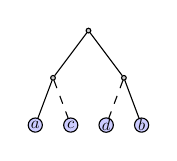
\begin{tikzpicture}[-,>=stealth', level/.style={sibling distance = 1.5cm/#1, level distance = 1cm}, scale=0.6,transform shape]

    \node {}
        child{
            node {}
                child{
                    node [main node] (a) {$a$}
                }
                child[edge from parent path = {(\tikzparentnode ) -- (\tikzchildnode) [dashed]}]{
                    node [main node] (b) {$c$}
                }
        }
        child{
            node {}
                child[edge from parent path = {(\tikzparentnode ) -- (\tikzchildnode) [dashed]}]{
                    node [main node] {$d$}
                }
                child{
                    node [main node] (d) {$b$}
                }
        }
    ;
    
\end{tikzpicture}



\end{document}